\documentclass[11pt,master]{oecu-thesis}
%\documentclass[11pt,draft]{oecu-thesis}% ドラフト(草稿)の場合は,
                               % 上の行をコメントアウトして,
                               % そのかわりにこの行を用いる.

\usepackage{times}
\usepackage[dvipdfmx]{graphicx}

\usepackage{url}
\usepackage{times}
\usepackage{multicol}
\usepackage{setspace}
\usepackage{comment}

%%% 自分の内容に合わせて書く.
\title{論文執筆にあたっての注意}
% 表紙のタイトルに改行を入れたい場合はその他のタイトルを次のように[]内に書く.
%\title[その他のタイトル]{表紙の\\タイトル}

\author{電通 太郎}
\date{2023年2月13日}
\学生番号{MT21A000}
\指導教員{大阪 次郎 教授}

%\論文種別{特別研究論文} % 特別研究の場合はコメントをはずす.
\年度{2022}
\専攻{総合情報学専攻}
\所属{コンピュータサイエンスコース}


%%% ▼補助的なコマンド (必要に応じて使う.)

% XMLなどの<abc>は\tag{abc}のように入力する.
\newcommand{\tag}[1]{$\langle$\nobreak#1\nobreak$\rangle$}

% UMLなどの<<abc>>は\stereotype{abc}のように入力する.
\newcommand{\stereotype}[1]{\raisebox{0.45ex}{$_\ll$}\nobreak
  #1\nobreak\raisebox{0.45ex}{$_\gg$}}

%%% ▲補助的なコマンドはここまで.


\begin{document}
\maketitle
\pagenumbering{roman}

\paperlist{%
  \begin{enumerate}
    \item あれや
    \item これや
    \item それや
  \end{enumerate}
}

\begin{abstract}

\begin{multicols}{2}
\small
\setlength{\parindent}{1zw}
\begin{spacing}{1.0}
ああああああああああああああああああああ
ああああああああああああああああああああ
ああああああああああああああああああああ
ああああああああああああああああああああ
ああああああああああああああああああああ
ああああああああああああああああああああ
ああああああああああああああああああああ
ああああああああああああああああああああ
ああああああああああああああああああああ
ああああああああああああああああああああ
ああああああああああああああああああああ
ああああああああああああああああああああ
ああああああああああああああああああああ
ああああああああああああああああああああ
ああああああああああああああああああああ
ああああああああああああああああああああ
ああああああああああああああああああああ
ああああああああああああああああああああ
ああああああああああああああああああああ
ああああああああああああああああああああ
ああああああああああああああああああああ
ああああああああああああああああああああ
ああああああああああああああああああああ
ああああああああああああああああああああ
ああああああああああああああああああああ
ああああああああああああああああああああ
ああああああああああああああああああああ
ああああああああああああああああああああ
ああああああああああああああああああああ
ああああああああああああああああああああ
ああああああああああああああああああああ
ああああああああああああああああああああ
ああああああああああああああああああああ
ああああああああああああああああああああ
ああああああああああああああああああああ
ああああああああああああああああああああ
ああああああああああああああああああああ
ああああああああああああああああああああ
ああああああああああああああああああああ
ああああああああああああああああああああ
ああああああああああああああああああああ
ああああああああああああああああああああ
ああああああああああああああああああああ
ああああああああああああああああああああ
ああああああああああああああああああああ
ああああああああああああああああああああ
ああああああああああああああああああああ
ああああああああああああああああああああ
ああああああああああああああああああああ
ああああああああああああああああああああ
ああああああああああああああああああああ
ああああああああああああああああああああ
ああああああああああああああああああああ
ああああああああああああああああああああ
ああああああああああああああああああああ
ああああああああああああああああああああ
ああああああああああああああああああああ
ああああああああああああああああああああ
ああああああああああああああああああああ
ああああああああああああああああああああ
ああああああああああああああああああああ
ああああああああああああああああああああ
ああああああああああああああああああああ
ああああああああああああああああああああ
ああああああああああああああああああああ
ああああああああああああああああああああ
ああああああああああああああああああああ
ああああああああああああああああああああ
ああああああああああああああああああああ
ああああああああああああああああああああ
ああああああああああああああああああああ
ああああああああああああああああああああ
ああああああああああああああああああああ
ああああああああああああああああああああ
ああああああああああああああああああああ
ああああああああああああああああああああ
ああああああああああああああああああああ
ああああああああああああああああああああ
ああああああああああああああああああああ
ああああああああああああああああああああ
ああああああああああああああああああああ
ああああああああああああああああああああ
ああああああああああああああああああああ
ああああああああああああああああああああ
ああああああああああああああああああああ
ああああああああああああああああああああ
ああああああああああああああああああああ
ああああああああああああああああああああ
ああああああああああああああああああああ
ああああああああああああああああああああ
ああああああああああああああああああああ
ああああああああああああああああああああ
ああああああああああああああああああああ
ああああああああああああああああああああ
ああああああああああああああああああああ
ああああああああああああああああああああ
ああああああああああああああああああああ
ああああああああああああああああああああ
ああああああああああああああああああああ
ああああああああああああああああああああ\\
(以上2000字)
\end{spacing}
\end{multicols}

\begin{comment}
  \comment{このようにコメントを書くと,ドラフトの場合に
  のみ表示される.}
「内容梗概」は,研究内容の要約である.つまり,研究では何
を行ったのか,研究の工夫点(キーアイデア),および,研究で
得られた知見を簡潔に表す.通常は,段落を分けることはせず,
一つの段落として記述する.内容梗概の重要な役割は,読み
手にとって,その論文の内容が読み手の興味を引く内容である
かどうかの判断材料となることである.逆に言えば,内容梗
概がきちんとまとめられていなければ,研究内容そのものも
否定的に見られることになる.よって,内容梗概の作成にあ
たっては,こういった点を考慮した上で十分推敲することが望
ましい.また,内容梗概に続く「主な用語」では,研究内容
で重要となる項目を,一般的な学術用語(キーワード)を列挙す
ることで表す.このとき,キーワードを見るだけで,研究の内
容がある程度推測できることが望ましい.主な用語は,通常5
個程度列挙する.

内容梗概は次の順に記述する.
\begin{enumerate}
\item 研究で何を行ったか.(1文) 「本研究では,〜した.」
\item 研究のねらい(新規性).(1文)      「〜できれば,〜なると期待できる.」
\item 研究の概要.(1文)        「考案した内容は,具体的には,〜である.」
                               または「本研究では,具体的には,〜した.」 
\item キーアイデアの記述.(数文)
\item 有効性に関する記述.(数文)
\item まとめ.(1文)            「これにより,〜といえる.」
\end{enumerate}

\keywords % 主な用語
  修士学位論文\quad 
  卒業論文\quad 
  基本構成\quad 
  注意点\quad 
  作文技法
\end{comment}
\end{abstract}

\newpage

\tableofcontents
\cleardoublepage

\setcounter{page}{1}
\pagenumbering{arabic}

\chapter{はじめに}\label{chap:intro}

「はじめに」は,研究の内容をアピールする章である.
つまり,研究でどんな問題を扱ったのか,なぜその問題を解
決する必要があるのか,その問題を解決することがどれだけ
重要か,どんな方法で解決したのか,どこまでできたのか,
結果として何がわかったのか,など,研究の意図が十分読み
手に伝わるように記述する.
したがって,悪い書き方の一例としては,すべて終わったわけではないのに問題をすべて解決
したかのように思われるような書き方がある.
ここで,注意が必要なのは,このような事実に反する記述を,
意図せずに行っている場合があることである.
つまり,書き手が表現したい内容と実際に書いた文に書かれて
いる内容が一致していないのである.
ここで重要なことは,自分の書いた文章を,自分の意図とは切り離し
て,素直に読んだ場合にどういう解釈になるのかを考えること
である.
基本的な文章の書き方の注意点については\cite{sakubun}など
を参照せよ.

「はじめに」で記述する項目は,具体的には次のとおりである.
\begin{itemize}
\item 研究の動機・位置づけ
\item 関連研究
\item 研究の内容(新規性・キーアイデア)
\item 得られた知見(有用性)
\item 論文の構成
\end{itemize}
ただし,特に節は設けず,各々の項目を段落に分けて記述する.

研究の動機・位置づけでは,研究で取り組んだ問題は何か,
現状ではどこまで解決されており,何が問題となっているのか,
などを明記する.

関連研究では,前段落で述べた問題へのアプローチとして,
世の中ではどのような解決策が考えられているのか,また,
問題の解決につながる可能性を持つ技術として,何が知られて
いるのか,などを記述する.これにともない,関連研究の内容
が分かる文献を文献リストに挙げる.

研究の内容では,自分がどのように問題を解決したのかを
より具体的に記述する.このとき,どこが新しいのか(新規性),
制限は何か(適用可能な範囲)を明記することが望ましい.

得られた知見では,研究成果として,どこまでできたのか,
また,何が言えるのか(有効性)を明らかにする.

以上の各項目の内容は,当然他の項目の内容と関連している.
すなわち,「問題点」とそれに対する「関連研究」,「関連研究」と
それとは違う新しい「研究内容」,「研究内容」とその「研究
成果」,「研究成果」と最初に挙げた「問題点」,と
いった関係である.これらの関係を,読み手が文章を読んだだ
けで理解できるようにすることが求められる.


論文の構成では,論文の話の流れが分かるように,各章の内容を
簡単に述べる.

本稿の構成は次のとおりである.まず,第\ref{chap:contents}章で
研究内容をどのように書いていけばよいか記述する.次に,
第\ref{chap:discussion}章で考察に書くべき内容について述べる.
その後,参考文献リストに挙げる文献の選び方を述べる.
最後に,おわりにでのまとめ方を述べる.

\chapter{研究内容の記述}\label{chap:contents}

第\ref{chap:intro}章「はじめに」の次の章からは,研究内容を記述する.
「はじめに」とは対象的に,客観的な事実を中心に書く.
つまり,「はじめに」で書いた内容が本当なのか判断できる
ように,正確かつ詳細に研究の内容を記述すればよい.

\section{研究内容を書く際の注意}

特に注意するべきことは,他人の成果,つまり,自分が行ったり考えたりしたことで
はないことを書く場合は,それが自分の研究とどう関係しているのかをあ
らかじめ記述しておくことである.悪い例としては,自分の行っ
ていない,予備的な知識を長々と書き,それが自分の研究とど
う関係しているのかを書かずに次の話題に移ってしまうような
書き方がある.卒業論文では,あくまで自分の行ったことを中
心として記述する.したがって,たとえ既存の技術や成果を利用していたとしても,
自分の研究の中でそれらがどう関係しているのかを明記する.

\section{章立て}

研究内容は,内容をもとに章を分ける.
更に,各章は適宜節に分ける.
通常は研究内容をいくつかの項目に分けて順に記述する方が分かり
やすい.このため,章や節に分けて記述するのである.
つまり,逆に言うと,もし同じ内容を複数の章や節で繰り返すと,
冗長になり,章や節に分けた意味がなくなってしまう.
そうならないように注意すること.

章や節の開始では,前の章との関連性や,その節で述べている
内容を簡単にまとめて記述するとよい.

\subsection{節の区切り方}

節の区切りで改頁してはならない.

\subsubsection{節の深さ}

節を深くしすぎてはならない.せいぜいsubsectionまでである.

\section{図・表}

図や表は読み手の理解を助けるために重要である.しかし,図
や表だけではその意図は読み手に正確認伝わるとは限らない.
このため,図や表を入れた場合,その図や表の各部分が何を表
すのかや,何を読み取って欲しいのかを本文中で説明する必要
がある.

図や表の入れ方は次のとおりである.
図や表は,必ず番号と見出し(キャプション)を付ける.
文と文の間には入れず,ページの上部に入れる.
大きい場合は一ページにしたり,更に複数のページを
用いてもよい.
図や表の文字は,本文の文字とのバランスを考え,
大きすぎたり小さすぎたりしないように調整する.
図\ref{fig:fontsize}や表\ref{tab:sample}のように,本文の文字の大きさか,少し
小さいくらいが適切な大きさである.

\begin{figure}[t]
  \begin{center}
    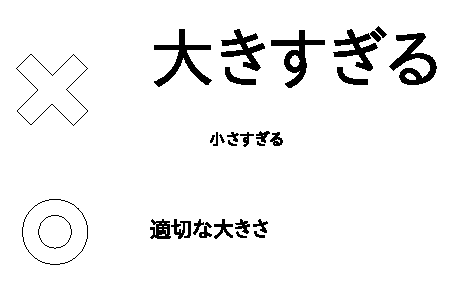
\includegraphics{samplefigure.eps}
    \caption{図中の文字の大きさ}\label{fig:fontsize}
  \end{center}
\end{figure}

\begin{table}[t]
  \caption{表の例}\label{tab:sample}
  \begin{center}
    \small
    \begin{tabular}{|c||c|c|}
      \hline
      表の例   & before & after \\
      \hline
      \hline
      this one & 3      & 5 \\
      \hline
      that one & N/A    &  --- \\
      \hline
    \end{tabular}
  \end{center}
\end{table}

\section{数式}

数式は理論などを正確に表現する際に用いる.ただし,式中の
文字の定義を書かずに数式だけを書くのは不十分である.また,
式の直観的な意味を説明することも必要である.

数式は$ y = ax + b$のように本文に埋め込む書き方と,次の
式(\ref{eqn:example})のように式を独立して書く書き方がある.
\begin{eqnarray}
f(n) & = & \sum^{n}_{i = 1}a_i \times (b_i - c_i) \label{eqn:example}
\end{eqnarray}
重要な式は,式(\ref{eqn:example})のように番号を付け,
本文ではその番号により参照する.

\chapter{考察}\label{chap:discussion}

「考察」では,研究成果として何が明らかになったのかを,
論理的に示す.論理的に示すためには,なぜそうなるのか,
それは正しいのか,といったことが判断できる客観的な事実を
挙げなければならない.記述する際には,特に,事実と自分の
意見(主張)とをきちんと区別して,それが分かるように表現し
なければならない.

考察の範囲は,残された問題点まで含める方がよい.単に問題
点を列挙するだけでなく,どのようにすればそれが解決できそ
うか,見通しを示す方がよい.

\chapter{参考文献リストに挙げる文献}\label{chap:ref}

研究内容と直接関係のない内容については,参考文献を示し,
その内容には本文中ではあまりふれない.

参考文献リストは,どこまで既存の成果を調査しているかの指
標になる.つまり,逆に考えると,参考文献リストにほとんど文
献が載っていない場合,何も調べていないように思われ,卒業
論文や修士学位論文の内容そのものもできが良くないと判断されることになる.

参考文献として挙げる文献の種類としては,論文誌の論文
\cite{kern99:fmv_survey}・国際会議や研究会などの論文
\cite{nML1995}などが望ましいが,書籍\cite{sakubun}やマニュ
アル\cite{CWL-LRM-1.1},ネットワーク上のウェブサイトや公
開文書\cite{systemc}なども挙げてよい.

\chapter{見直し}

分かりやすい文章にするためには,見直しが必要である.

見直しは印刷して行う.
基本的なこととして,誤字・脱字などがないかや主語と述語がきちんと対応しているかな
どを確認する.
さらに,書かれている内容を可能な限り文字通りに解釈し,自分の言
いたいことと書かれている内容とが一致しているかや,あいま
いな表現になっていないかを判断する.
それに加えて,論理的な飛躍や抜けがないかを確かめる.

黙読だけでなく,音読も行う.
音読したときに句の切れ目や文の意味などがすぐに判断できない文は,悪い文である.
悪い文は,わかりやすい文に変更する.

他人に読んでもらったり聞いてもらったりす
ると,どこが悪いのかがわかりやすい.

\chapter{おわりに}

「おわりに」では,あらためて,研究で何を行ったのか,また,そ
の成果は何か,を簡潔にまとめる.また,今後の課題も簡潔にまとめる.
特に,今後の課題については,たくさんある場合でも,あまり多
くは書かず,次にするべきことは何かを簡潔にまとめる.
今後の課題がたくさんある場合には,考察のところで取り上げ,
どのようなアプローチが考えられるかをなるべく具体的に書く
とよい.


\acknowledgment

「謝辞」では,卒業研究や修士の研究でお世話になった先生や
先輩に対して感謝の意を表す.卒業研究や修士の研究とはいう
ものの,大学や大学院で得た知識の集大成が卒業研究や修士の
研究の成果なのであるから,それをふまえて,広く感謝の意を
表す方がよい.

通常,謝辞では,感謝の度合が高いほど先に書く.また,何
人かを一まとめにするよりは,個別に謝辞を書く方が,感謝の
度合が高くなる.同列に並べる時でも,役職の高い人を先に書
くなど,一般的に常識とされることがあるので,気を配った方
がよい.

\bibliographystyle{junsrt}
\bibliography{samplebib}

\appendix
\chapter{付録として付けることがら}

付録では実験の全データやプログラムリストなどを付ける.
他の人が同じ実験やプログラムの実行ができるようにする.
付録にも,章や節を付ける.

研究に直接関係することは付録にせずに本文に書く.
\end{document}
